\documentclass{article}
\usepackage{iclr2027_conference,times}
%%%%% NEW MATH DEFINITIONS %%%%%

\usepackage{amsmath,amsfonts,bm}

% Mark sections of captions for referring to divisions of figures
\newcommand{\figleft}{{\em (Left)}}
\newcommand{\figcenter}{{\em (Center)}}
\newcommand{\figright}{{\em (Right)}}
\newcommand{\figtop}{{\em (Top)}}
\newcommand{\figbottom}{{\em (Bottom)}}
\newcommand{\captiona}{{\em (a)}}
\newcommand{\captionb}{{\em (b)}}
\newcommand{\captionc}{{\em (c)}}
\newcommand{\captiond}{{\em (d)}}

% Highlight a newly defined term
\newcommand{\newterm}[1]{{\bf #1}}


% Figure reference, lower-case.
\def\figref#1{figure~\ref{#1}}
% Figure reference, capital. For start of sentence
\def\Figref#1{Figure~\ref{#1}}
\def\twofigref#1#2{figures \ref{#1} and \ref{#2}}
\def\quadfigref#1#2#3#4{figures \ref{#1}, \ref{#2}, \ref{#3} and \ref{#4}}
% Section reference, lower-case.
\def\secref#1{section~\ref{#1}}
% Section reference, capital.
\def\Secref#1{Section~\ref{#1}}
% Reference to two sections.
\def\twosecrefs#1#2{sections \ref{#1} and \ref{#2}}
% Reference to three sections.
\def\secrefs#1#2#3{sections \ref{#1}, \ref{#2} and \ref{#3}}
% Reference to an equation, lower-case.
\def\eqref#1{equation~\ref{#1}}
% Reference to an equation, upper case
\def\Eqref#1{Equation~\ref{#1}}
% A raw reference to an equation---avoid using if possible
\def\plaineqref#1{\ref{#1}}
% Reference to a chapter, lower-case.
\def\chapref#1{chapter~\ref{#1}}
% Reference to an equation, upper case.
\def\Chapref#1{Chapter~\ref{#1}}
% Reference to a range of chapters
\def\rangechapref#1#2{chapters\ref{#1}--\ref{#2}}
% Reference to an algorithm, lower-case.
\def\algref#1{algorithm~\ref{#1}}
% Reference to an algorithm, upper case.
\def\Algref#1{Algorithm~\ref{#1}}
\def\twoalgref#1#2{algorithms \ref{#1} and \ref{#2}}
\def\Twoalgref#1#2{Algorithms \ref{#1} and \ref{#2}}
% Reference to a part, lower case
\def\partref#1{part~\ref{#1}}
% Reference to a part, upper case
\def\Partref#1{Part~\ref{#1}}
\def\twopartref#1#2{parts \ref{#1} and \ref{#2}}

\def\ceil#1{\lceil #1 \rceil}
\def\floor#1{\lfloor #1 \rfloor}
\def\1{\bm{1}}
\newcommand{\train}{\mathcal{D}}
\newcommand{\valid}{\mathcal{D_{\mathrm{valid}}}}
\newcommand{\test}{\mathcal{D_{\mathrm{test}}}}

\def\eps{{\epsilon}}


% Random variables
\def\reta{{\textnormal{$\eta$}}}
\def\ra{{\textnormal{a}}}
\def\rb{{\textnormal{b}}}
\def\rc{{\textnormal{c}}}
\def\rd{{\textnormal{d}}}
\def\re{{\textnormal{e}}}
\def\rf{{\textnormal{f}}}
\def\rg{{\textnormal{g}}}
\def\rh{{\textnormal{h}}}
\def\ri{{\textnormal{i}}}
\def\rj{{\textnormal{j}}}
\def\rk{{\textnormal{k}}}
\def\rl{{\textnormal{l}}}
% rm is already a command, just don't name any random variables m
\def\rn{{\textnormal{n}}}
\def\ro{{\textnormal{o}}}
\def\rp{{\textnormal{p}}}
\def\rq{{\textnormal{q}}}
\def\rr{{\textnormal{r}}}
\def\rs{{\textnormal{s}}}
\def\rt{{\textnormal{t}}}
\def\ru{{\textnormal{u}}}
\def\rv{{\textnormal{v}}}
\def\rw{{\textnormal{w}}}
\def\rx{{\textnormal{x}}}
\def\ry{{\textnormal{y}}}
\def\rz{{\textnormal{z}}}

% Random vectors
\def\rvepsilon{{\mathbf{\epsilon}}}
\def\rvtheta{{\mathbf{\theta}}}
\def\rva{{\mathbf{a}}}
\def\rvb{{\mathbf{b}}}
\def\rvc{{\mathbf{c}}}
\def\rvd{{\mathbf{d}}}
\def\rve{{\mathbf{e}}}
\def\rvf{{\mathbf{f}}}
\def\rvg{{\mathbf{g}}}
\def\rvh{{\mathbf{h}}}
\def\rvu{{\mathbf{i}}}
\def\rvj{{\mathbf{j}}}
\def\rvk{{\mathbf{k}}}
\def\rvl{{\mathbf{l}}}
\def\rvm{{\mathbf{m}}}
\def\rvn{{\mathbf{n}}}
\def\rvo{{\mathbf{o}}}
\def\rvp{{\mathbf{p}}}
\def\rvq{{\mathbf{q}}}
\def\rvr{{\mathbf{r}}}
\def\rvs{{\mathbf{s}}}
\def\rvt{{\mathbf{t}}}
\def\rvu{{\mathbf{u}}}
\def\rvv{{\mathbf{v}}}
\def\rvw{{\mathbf{w}}}
\def\rvx{{\mathbf{x}}}
\def\rvy{{\mathbf{y}}}
\def\rvz{{\mathbf{z}}}

% Elements of random vectors
\def\erva{{\textnormal{a}}}
\def\ervb{{\textnormal{b}}}
\def\ervc{{\textnormal{c}}}
\def\ervd{{\textnormal{d}}}
\def\erve{{\textnormal{e}}}
\def\ervf{{\textnormal{f}}}
\def\ervg{{\textnormal{g}}}
\def\ervh{{\textnormal{h}}}
\def\ervi{{\textnormal{i}}}
\def\ervj{{\textnormal{j}}}
\def\ervk{{\textnormal{k}}}
\def\ervl{{\textnormal{l}}}
\def\ervm{{\textnormal{m}}}
\def\ervn{{\textnormal{n}}}
\def\ervo{{\textnormal{o}}}
\def\ervp{{\textnormal{p}}}
\def\ervq{{\textnormal{q}}}
\def\ervr{{\textnormal{r}}}
\def\ervs{{\textnormal{s}}}
\def\ervt{{\textnormal{t}}}
\def\ervu{{\textnormal{u}}}
\def\ervv{{\textnormal{v}}}
\def\ervw{{\textnormal{w}}}
\def\ervx{{\textnormal{x}}}
\def\ervy{{\textnormal{y}}}
\def\ervz{{\textnormal{z}}}

% Random matrices
\def\rmA{{\mathbf{A}}}
\def\rmB{{\mathbf{B}}}
\def\rmC{{\mathbf{C}}}
\def\rmD{{\mathbf{D}}}
\def\rmE{{\mathbf{E}}}
\def\rmF{{\mathbf{F}}}
\def\rmG{{\mathbf{G}}}
\def\rmH{{\mathbf{H}}}
\def\rmI{{\mathbf{I}}}
\def\rmJ{{\mathbf{J}}}
\def\rmK{{\mathbf{K}}}
\def\rmL{{\mathbf{L}}}
\def\rmM{{\mathbf{M}}}
\def\rmN{{\mathbf{N}}}
\def\rmO{{\mathbf{O}}}
\def\rmP{{\mathbf{P}}}
\def\rmQ{{\mathbf{Q}}}
\def\rmR{{\mathbf{R}}}
\def\rmS{{\mathbf{S}}}
\def\rmT{{\mathbf{T}}}
\def\rmU{{\mathbf{U}}}
\def\rmV{{\mathbf{V}}}
\def\rmW{{\mathbf{W}}}
\def\rmX{{\mathbf{X}}}
\def\rmY{{\mathbf{Y}}}
\def\rmZ{{\mathbf{Z}}}

% Elements of random matrices
\def\ermA{{\textnormal{A}}}
\def\ermB{{\textnormal{B}}}
\def\ermC{{\textnormal{C}}}
\def\ermD{{\textnormal{D}}}
\def\ermE{{\textnormal{E}}}
\def\ermF{{\textnormal{F}}}
\def\ermG{{\textnormal{G}}}
\def\ermH{{\textnormal{H}}}
\def\ermI{{\textnormal{I}}}
\def\ermJ{{\textnormal{J}}}
\def\ermK{{\textnormal{K}}}
\def\ermL{{\textnormal{L}}}
\def\ermM{{\textnormal{M}}}
\def\ermN{{\textnormal{N}}}
\def\ermO{{\textnormal{O}}}
\def\ermP{{\textnormal{P}}}
\def\ermQ{{\textnormal{Q}}}
\def\ermR{{\textnormal{R}}}
\def\ermS{{\textnormal{S}}}
\def\ermT{{\textnormal{T}}}
\def\ermU{{\textnormal{U}}}
\def\ermV{{\textnormal{V}}}
\def\ermW{{\textnormal{W}}}
\def\ermX{{\textnormal{X}}}
\def\ermY{{\textnormal{Y}}}
\def\ermZ{{\textnormal{Z}}}

% Vectors
\def\vzero{{\bm{0}}}
\def\vone{{\bm{1}}}
\def\vmu{{\bm{\mu}}}
\def\vtheta{{\bm{\theta}}}
\def\va{{\bm{a}}}
\def\vb{{\bm{b}}}
\def\vc{{\bm{c}}}
\def\vd{{\bm{d}}}
\def\ve{{\bm{e}}}
\def\vf{{\bm{f}}}
\def\vg{{\bm{g}}}
\def\vh{{\bm{h}}}
\def\vi{{\bm{i}}}
\def\vj{{\bm{j}}}
\def\vk{{\bm{k}}}
\def\vl{{\bm{l}}}
\def\vm{{\bm{m}}}
\def\vn{{\bm{n}}}
\def\vo{{\bm{o}}}
\def\vp{{\bm{p}}}
\def\vq{{\bm{q}}}
\def\vr{{\bm{r}}}
\def\vs{{\bm{s}}}
\def\vt{{\bm{t}}}
\def\vu{{\bm{u}}}
\def\vv{{\bm{v}}}
\def\vw{{\bm{w}}}
\def\vx{{\bm{x}}}
\def\vy{{\bm{y}}}
\def\vz{{\bm{z}}}

% Elements of vectors
\def\evalpha{{\alpha}}
\def\evbeta{{\beta}}
\def\evepsilon{{\epsilon}}
\def\evlambda{{\lambda}}
\def\evomega{{\omega}}
\def\evmu{{\mu}}
\def\evpsi{{\psi}}
\def\evsigma{{\sigma}}
\def\evtheta{{\theta}}
\def\eva{{a}}
\def\evb{{b}}
\def\evc{{c}}
\def\evd{{d}}
\def\eve{{e}}
\def\evf{{f}}
\def\evg{{g}}
\def\evh{{h}}
\def\evi{{i}}
\def\evj{{j}}
\def\evk{{k}}
\def\evl{{l}}
\def\evm{{m}}
\def\evn{{n}}
\def\evo{{o}}
\def\evp{{p}}
\def\evq{{q}}
\def\evr{{r}}
\def\evs{{s}}
\def\evt{{t}}
\def\evu{{u}}
\def\evv{{v}}
\def\evw{{w}}
\def\evx{{x}}
\def\evy{{y}}
\def\evz{{z}}

% Matrix
\def\mA{{\bm{A}}}
\def\mB{{\bm{B}}}
\def\mC{{\bm{C}}}
\def\mD{{\bm{D}}}
\def\mE{{\bm{E}}}
\def\mF{{\bm{F}}}
\def\mG{{\bm{G}}}
\def\mH{{\bm{H}}}
\def\mI{{\bm{I}}}
\def\mJ{{\bm{J}}}
\def\mK{{\bm{K}}}
\def\mL{{\bm{L}}}
\def\mM{{\bm{M}}}
\def\mN{{\bm{N}}}
\def\mO{{\bm{O}}}
\def\mP{{\bm{P}}}
\def\mQ{{\bm{Q}}}
\def\mR{{\bm{R}}}
\def\mS{{\bm{S}}}
\def\mT{{\bm{T}}}
\def\mU{{\bm{U}}}
\def\mV{{\bm{V}}}
\def\mW{{\bm{W}}}
\def\mX{{\bm{X}}}
\def\mY{{\bm{Y}}}
\def\mZ{{\bm{Z}}}
\def\mBeta{{\bm{\beta}}}
\def\mPhi{{\bm{\Phi}}}
\def\mLambda{{\bm{\Lambda}}}
\def\mSigma{{\bm{\Sigma}}}

% Tensor
\DeclareMathAlphabet{\mathsfit}{\encodingdefault}{\sfdefault}{m}{sl}
\SetMathAlphabet{\mathsfit}{bold}{\encodingdefault}{\sfdefault}{bx}{n}
\newcommand{\tens}[1]{\bm{\mathsfit{#1}}}
\def\tA{{\tens{A}}}
\def\tB{{\tens{B}}}
\def\tC{{\tens{C}}}
\def\tD{{\tens{D}}}
\def\tE{{\tens{E}}}
\def\tF{{\tens{F}}}
\def\tG{{\tens{G}}}
\def\tH{{\tens{H}}}
\def\tI{{\tens{I}}}
\def\tJ{{\tens{J}}}
\def\tK{{\tens{K}}}
\def\tL{{\tens{L}}}
\def\tM{{\tens{M}}}
\def\tN{{\tens{N}}}
\def\tO{{\tens{O}}}
\def\tP{{\tens{P}}}
\def\tQ{{\tens{Q}}}
\def\tR{{\tens{R}}}
\def\tS{{\tens{S}}}
\def\tT{{\tens{T}}}
\def\tU{{\tens{U}}}
\def\tV{{\tens{V}}}
\def\tW{{\tens{W}}}
\def\tX{{\tens{X}}}
\def\tY{{\tens{Y}}}
\def\tZ{{\tens{Z}}}


% Graph
\def\gA{{\mathcal{A}}}
\def\gB{{\mathcal{B}}}
\def\gC{{\mathcal{C}}}
\def\gD{{\mathcal{D}}}
\def\gE{{\mathcal{E}}}
\def\gF{{\mathcal{F}}}
\def\gG{{\mathcal{G}}}
\def\gH{{\mathcal{H}}}
\def\gI{{\mathcal{I}}}
\def\gJ{{\mathcal{J}}}
\def\gK{{\mathcal{K}}}
\def\gL{{\mathcal{L}}}
\def\gM{{\mathcal{M}}}
\def\gN{{\mathcal{N}}}
\def\gO{{\mathcal{O}}}
\def\gP{{\mathcal{P}}}
\def\gQ{{\mathcal{Q}}}
\def\gR{{\mathcal{R}}}
\def\gS{{\mathcal{S}}}
\def\gT{{\mathcal{T}}}
\def\gU{{\mathcal{U}}}
\def\gV{{\mathcal{V}}}
\def\gW{{\mathcal{W}}}
\def\gX{{\mathcal{X}}}
\def\gY{{\mathcal{Y}}}
\def\gZ{{\mathcal{Z}}}

% Sets
\def\sA{{\mathbb{A}}}
\def\sB{{\mathbb{B}}}
\def\sC{{\mathbb{C}}}
\def\sD{{\mathbb{D}}}
% Don't use a set called E, because this would be the same as our symbol
% for expectation.
\def\sF{{\mathbb{F}}}
\def\sG{{\mathbb{G}}}
\def\sH{{\mathbb{H}}}
\def\sI{{\mathbb{I}}}
\def\sJ{{\mathbb{J}}}
\def\sK{{\mathbb{K}}}
\def\sL{{\mathbb{L}}}
\def\sM{{\mathbb{M}}}
\def\sN{{\mathbb{N}}}
\def\sO{{\mathbb{O}}}
\def\sP{{\mathbb{P}}}
\def\sQ{{\mathbb{Q}}}
\def\sR{{\mathbb{R}}}
\def\sS{{\mathbb{S}}}
\def\sT{{\mathbb{T}}}
\def\sU{{\mathbb{U}}}
\def\sV{{\mathbb{V}}}
\def\sW{{\mathbb{W}}}
\def\sX{{\mathbb{X}}}
\def\sY{{\mathbb{Y}}}
\def\sZ{{\mathbb{Z}}}

% Entries of a matrix
\def\emLambda{{\Lambda}}
\def\emA{{A}}
\def\emB{{B}}
\def\emC{{C}}
\def\emD{{D}}
\def\emE{{E}}
\def\emF{{F}}
\def\emG{{G}}
\def\emH{{H}}
\def\emI{{I}}
\def\emJ{{J}}
\def\emK{{K}}
\def\emL{{L}}
\def\emM{{M}}
\def\emN{{N}}
\def\emO{{O}}
\def\emP{{P}}
\def\emQ{{Q}}
\def\emR{{R}}
\def\emS{{S}}
\def\emT{{T}}
\def\emU{{U}}
\def\emV{{V}}
\def\emW{{W}}
\def\emX{{X}}
\def\emY{{Y}}
\def\emZ{{Z}}
\def\emSigma{{\Sigma}}

% entries of a tensor
% Same font as tensor, without \bm wrapper
\newcommand{\etens}[1]{\mathsfit{#1}}
\def\etLambda{{\etens{\Lambda}}}
\def\etA{{\etens{A}}}
\def\etB{{\etens{B}}}
\def\etC{{\etens{C}}}
\def\etD{{\etens{D}}}
\def\etE{{\etens{E}}}
\def\etF{{\etens{F}}}
\def\etG{{\etens{G}}}
\def\etH{{\etens{H}}}
\def\etI{{\etens{I}}}
\def\etJ{{\etens{J}}}
\def\etK{{\etens{K}}}
\def\etL{{\etens{L}}}
\def\etM{{\etens{M}}}
\def\etN{{\etens{N}}}
\def\etO{{\etens{O}}}
\def\etP{{\etens{P}}}
\def\etQ{{\etens{Q}}}
\def\etR{{\etens{R}}}
\def\etS{{\etens{S}}}
\def\etT{{\etens{T}}}
\def\etU{{\etens{U}}}
\def\etV{{\etens{V}}}
\def\etW{{\etens{W}}}
\def\etX{{\etens{X}}}
\def\etY{{\etens{Y}}}
\def\etZ{{\etens{Z}}}

% The true underlying data generating distribution
\newcommand{\pdata}{p_{\rm{data}}}
% The empirical distribution defined by the training set
\newcommand{\ptrain}{\hat{p}_{\rm{data}}}
\newcommand{\Ptrain}{\hat{P}_{\rm{data}}}
% The model distribution
\newcommand{\pmodel}{p_{\rm{model}}}
\newcommand{\Pmodel}{P_{\rm{model}}}
\newcommand{\ptildemodel}{\tilde{p}_{\rm{model}}}
% Stochastic autoencoder distributions
\newcommand{\pencode}{p_{\rm{encoder}}}
\newcommand{\pdecode}{p_{\rm{decoder}}}
\newcommand{\precons}{p_{\rm{reconstruct}}}

\newcommand{\laplace}{\mathrm{Laplace}} % Laplace distribution

\newcommand{\E}{\mathbb{E}}
\newcommand{\Ls}{\mathcal{L}}
\newcommand{\R}{\mathbb{R}}
\newcommand{\emp}{\tilde{p}}
\newcommand{\lr}{\alpha}
\newcommand{\reg}{\lambda}
\newcommand{\rect}{\mathrm{rectifier}}
\newcommand{\softmax}{\mathrm{softmax}}
\newcommand{\sigmoid}{\sigma}
\newcommand{\softplus}{\zeta}
\newcommand{\KL}{D_{\mathrm{KL}}}
\newcommand{\Var}{\mathrm{Var}}
\newcommand{\standarderror}{\mathrm{SE}}
\newcommand{\Cov}{\mathrm{Cov}}
% Wolfram Mathworld says $L^2$ is for function spaces and $\ell^2$ is for vectors
% But then they seem to use $L^2$ for vectors throughout the site, and so does
% wikipedia.
\newcommand{\normlzero}{L^0}
\newcommand{\normlone}{L^1}
\newcommand{\normltwo}{L^2}
\newcommand{\normlp}{L^p}
\newcommand{\normmax}{L^\infty}

\newcommand{\parents}{Pa} % See usage in notation.tex. Chosen to match Daphne's book.

\DeclareMathOperator*{\argmax}{arg\,max}
\DeclareMathOperator*{\argmin}{arg\,min}

\DeclareMathOperator{\sign}{sign}
\DeclareMathOperator{\Tr}{Tr}
\let\ab\allowbreak

\usepackage{hyperref}
\usepackage{url}
\usepackage{graphicx}
\usepackage{booktabs}
\usepackage{amsmath,amssymb,amsthm}
\usepackage{xcolor}
\usepackage{multirow}
\usepackage{tikz}
\usetikzlibrary{arrows.meta,positioning,calc,shapes.geometric,fit,backgrounds}
\usepackage{algorithm}
\usepackage{algpseudocode}
\usepackage{caption}
\newcommand{\pending}[1]{\textcolor{blue!70!black}{[#1]}}
\newtheorem{proposition}{Proposition}
\newtheorem{definition}{Definition}
\newtheorem{assumption}{Assumption}
\newcommand{\Uz}[1]{U_{#1}}
\newcommand{\pww}{p_{\mathrm{ww}}}
\newcommand{\pcw}{p_{\mathrm{cw}}}
\newcommand{\piinf}{\pi_{\infty}}
\definecolor{cue}{RGB}{185,28,28}\definecolor{evid}{RGB}{21,128,61}\definecolor{rel}{RGB}{29,78,216}\definecolor{ink}{RGB}{40,44,52}\definecolor{soft}{RGB}{238,241,245}

\title{Confidence Without Control: Language Models Know\\When They Might Be Wrong and Revise Anyway}

\author{Anonymous authors\\Paper under double-blind review}

%\iclrfinalcopy
\begin{document}
\maketitle

\begin{abstract}
Language models maintain increasingly accurate estimates of whether their own answers are correct, yet those estimates exert almost no control over what the models do when a user pushes back. We name this dissociation the confidence-use gap, give it a normative benchmark and a price, and measure both of its sides across nineteen post-training checkpoints from five families, two current-generation models, and roughly 500{,}000 controlled trials. On the monitoring side, four independent uncertainty signals all predict the model's own correctness (AUROC up to 0.74 on hard questions) and the verbalized signal improves with scale (0.49 to 0.70). On the control side, a confound-free three-cell design in which wrong answers are challenged with \emph{different} wrong answers shows that models adopt an alternative they believe less than their current answer 90 to 99.5 percent of the time whenever the challenge carries a source cue; the model's own belief margin changes behaviour by at most 0.02 in all six models. A pooled regression over 44{,}629 trials quantifies the policy: being challenged sets revision near 0.9, the truth of the model's own claim moves it by 0.13, and its stated confidence by 0.02 per standard deviation. A pre-registered control shows that an apparent self-versus-other asymmetry is position, not source. One assumption predicts all of this: the trained policy is the corpus conditional of revision on visible context, and private reliability is never visible. It predicts that surfacing confidence cannot close the gap (confirmed: largest effect 0.069, no dose-response), that demonstrations can (roughly 3{,}000 examples install near-perfect rule-following at three points of benchmark cost against the untrained base and zero against a matched control), and that a forwarded answer acts on the next agent as a cue: across four open models an agent abandons a correct answer 80--89 percent of the time when a peer names an alternative, whether the peer is weaker, the same, or stronger, and a wrong answer forwarded through eight agents is retained with probability 0.98 per hop, so any answer-passing pipeline converges to an error rate set by drift alone (0.67--0.92). The propagation dynamics have a closed form, machine-checked in Lean, with three consequences for system design: consensus among such agents measures the cue rather than the truth, adding agents makes a wrong majority wronger, and a correct minority answer survives only in agents that never see the others.
\end{abstract}

\section{Introduction}
Ask a strong open-weight model a factual question and it answers correctly most of the time. Tell it, with no evidence whatsoever, that another source disagrees, and a seven-billion-parameter model abandons roughly half of the answers it had just gotten right. The literature calls this sycophancy \citep{sharma2023sycophancy,perez2022discovering}. This paper asks a different question. A rational reviser deciding whether to keep or change an answer should consult two quantities: how confident it was in the original answer, and how much evidence the challenge carries. Modern language models demonstrably possess the first quantity; a decade of calibration work has established that they can report when they are likely to be wrong \citep{kadavath2022language}. Do they use it when it matters?

They do not, and we measure that from enough directions to treat it as a basic property of current post-trained models rather than a quirk of any protocol. \textbf{Monitoring is good and improving}: verbalized confidence discriminates a model's own correct from incorrect answers with AUROC rising from 0.49 at 1.5B to 0.70 at 14B on the Qwen2.5 ladder, and verbalized confidence, $P(\mathrm{True})$ self-evaluation and a clean-context belief score all reach 0.60--0.74 across six models including a 2025-generation model and a reasoning-distilled one. \textbf{Control ignores the monitor}: in a design that removes a confound present in prior work (Section~\ref{sec:control}), models adopt an alternative they believe \emph{less} than their current answer 90 to 99.5 percent of the time when the challenge mentions a source; the belief margin between the two answers shifts the decision by at most 0.02, and stated confidence by 0.02 per standard deviation. What sets the operating point is the act of being challenged. The cognitive science of metacognition draws exactly this distinction between monitoring and control and treats their coupling as the point of having a monitor \citep{nelson1990metamemory}; the calibration literature has implicitly assumed the coupling. Our results say it does not hold.

Section~\ref{sec:framework} makes the gap precise and says why it exists. A Bayesian reviser must be moved by a calibrated reliability signal (Proposition~\ref{prop:bayes}), and ignoring it costs a computable amount of post-challenge accuracy (Proposition~\ref{prop:regret}). One assumption about the training objective, that a policy fit by cross-entropy to human dialogue becomes the corpus conditional of revision on \emph{visible} context, predicts the gap, predicts that it widens with scale, predicts that surfacing confidence as a token cannot close it while demonstrations can, and predicts one more thing with consequences beyond a single chat: a forwarded answer in a multi-agent pipeline is a visible cue, so contamination should propagate as a composition of the single-model policy and should not depend on who sent it. Section~\ref{sec:agents} confirms this on chains of eight agents, fits the closed-form dynamics of Proposition~\ref{prop:chain}, and derives the design rules that follow.

\paragraph{Contributions.} (i) The confidence-use gap as a measured quantity distinct from calibration, with a normative benchmark, a price, and one mechanism that predicts every result below; the propagation dynamics are machine-checked. (ii) An identification design that separates ``switches to the true answer'' from ``switches to whatever was named'', a pooled policy estimate, two nulls (surfacing, instruction) and a pre-registered reversal that the conformity literature needs. (iii) The installation half: demonstrations install rule-following at approximately zero marginal capability price, and a bidirectional intervention installs and removes capitulation; \pending{the public preference recipe and a correctness-rewarded arm}. (iv) The first test of answer contamination between agents as a composition of the single-model policy, on four models, with sender-competence invariance, an eight-hop chain measurement, and the rules it implies for multi-agent systems. (v) A free instrument: survival under challenge out-predicts stated confidence in sixteen of nineteen checkpoints.

\section{The gap, made precise}\label{sec:framework}
Let $c$ be a claim the assistant holds as its answer to question $q$ and $x$ a subsequent turn. A model that treated $x$ as evidence would revise according to
$\log\frac{P(c\ \mathrm{correct}\mid x,h)}{P(c\ \mathrm{incorrect}\mid x,h)}=\operatorname{logit}(r)+\log\ell(x)$,
where $r$ is the model's own reliability on $c$ and $\ell(x)$ the likelihood ratio the challenge carries. We decompose a turn into \textcolor{cue}{surface cues} $s(x)$ (an alternative is named, doubt is expressed, a source is invoked, the cue's position), \textcolor{evid}{evidence} $e(x)$, and \textcolor{rel}{own reliability} $r$, and write the revision policy $\pi(c,x)=\Pr[\text{switch}\mid c,x]$.

\begin{definition}[Behavioural use]\label{def:use}
For a signal $z\in\{s,e,r\}$, $\Uz{z}=\mathbb{E}[\pi\mid z_{\mathrm{lo}}]-\mathbb{E}[\pi\mid z_{\mathrm{hi}}]$ with the other two held fixed by design. Observational contrasts are reported separately, as associations.
\end{definition}
\begin{proposition}[A calibrated signal must move a Bayesian reviser]\label{prop:bayes}
Fix $\ell$. For $r_{\mathrm{lo}}<r_{\mathrm{hi}}$ with $\ell\in\big(\tfrac{r_{\mathrm{lo}}}{1-r_{\mathrm{lo}}},\tfrac{r_{\mathrm{hi}}}{1-r_{\mathrm{hi}}}\big)$, a non-empty band, the Bayesian policy switches at $r_{\mathrm{lo}}$ and holds at $r_{\mathrm{hi}}$; hence $\Uz{r}=1$ on the band.
\end{proposition}
\begin{proposition}[The accuracy cost of cue-following]\label{prop:regret}
For a content-free challenge on a two-candidate item, a reviser with calibrated reliability $r$ and pre-challenge accuracy $A=\mathbb{E}[r]$, and a cue-following policy that switches with probability $\pi$ independently of $r$,
$\;\mathbb{E}[\max(r,1-r)]-\big((1-\pi)A+\pi(1-A)\big)=\mathbb{E}[(1-2r)^{+}]+\pi\,(2A-1).$
\end{proposition}
\begin{proof}Holding yields $r$, switching $1-r$; take $\max$ pointwise for Bayes, the $\pi$-mixture for the cue-follower, subtract, and take expectations.\end{proof}
The first term is the value of using reliability at all; the second is the price of the cue: for a model that is right more often than not, every unit of cue-driven switching on an evidence-free challenge costs $2A-1$ in accuracy, and nothing in the challenge can pay for it. For Qwen2.5-7B on our hard bank ($A=0.87$) with the measured $\pi=0.63$ under content-free pressure, that is $0.47$.

\begin{assumption}[Corpus conditional]\label{ass:corpus}
Pretraining and supervised fine-tuning minimise cross-entropy on human dialogue, so in the limit $\pi(c,x)\to\Pr_{\mathrm{corpus}}[\mathrm{revise}\mid\mathrm{visible}(c,x)]$. Private reliability is not visible, and stated confidence in text is cheap talk.
\end{assumption}
Six predictions follow, each tested below. \textbf{P-flat}: $\Uz{r}\approx0$ regardless of calibration, and the gap widens with scale because capacity sharpens the fit to a conditional that lacks the private variable (\S\ref{sec:monitor}--\ref{sec:control}). \textbf{P-cue}: what is visible in the turn, a named alternative or a source-shaped sentence, sets the operating point; the truth of the alternative does not (\S\ref{sec:control}). \textbf{P-recency}: position is visible, speaker is not once position is matched (\S\ref{sec:control}). \textbf{P-surfacing}: writing $r$ into the context does not create $\Uz{r}$; only training that rewrites the conditional can (\S\ref{sec:control}, \S\ref{sec:install}). \textbf{P-training}: agreement-rewarded stages sharpen capitulation; demonstration- or correctness-rewarded stages reverse it (\S\ref{sec:install}). \textbf{P-propagation}: a forwarded answer is a cue, so contamination between agents is sender-invariant and Markov (\S\ref{sec:agents}).

\begin{proposition}[Chain dynamics]\label{prop:chain}
Let agent $k{+}1$ condition on the reply it receives, with $\pww=\Pr[\mathrm{wrong}_{k+1}\mid\mathrm{wrong}_k]$ and $\pcw=\Pr[\mathrm{wrong}_{k+1}\mid\mathrm{right}_k]$, $\pcw+1-\pww\neq0$. Then $\pi_k=\piinf+(\pi_1-\piinf)\lambda^{k-1}$ with $\lambda=\pww-\pcw$ and $\piinf=\pcw/(\pcw+1-\pww)$; $\piinf$ is the unique fixed point; the seed's influence decays geometrically when $0<\pcw<\pww\le1$; a fully contaminated chain arriving at an agent with retention $q$ restarts at $q$; and with a fraction $f$ of such agents the stationary error $\pcw/(\pcw+1-[(1-f)\pww+fq])$ is strictly decreasing in $f$ when $q<\pww$.
\end{proposition}
The proof is by induction on hops and is machine-checked (Appendix~\ref{app:lean}); the check caught a gap in an earlier draft that stated decay under $\pcw\ge0$. For $m$ independent chains combined by majority vote, $\Pr[\mathrm{majority\ wrong}]=\Pr[\mathrm{Bin}(m,\pi_k)>m/2]$ increases in $m$ whenever $\pi_k>\tfrac12$.

\section{Experimental setup}\label{sec:setup}
\paragraph{Banks.} 900 forced-choice items (600 MMLU-Pro \citep{wang2024mmlupro}, 300 TruthfulQA \citep{lin2022truthfulqa}) with a gold answer and one strong distractor; a 500-item identification bank with two distractors per item; 600 SciQ items \citep{welbl2017sciq} for training only. Every measurement uses held-out items that no training run sees.
\paragraph{Protocol.} A system prompt asks for a final line \texttt{FINAL: <answer>}. Turn 1: the question. Turn 2: the claim as the assistant's own prior turn (or, in the matched-position control, a user statement acknowledged by the assistant). Turn 3: the challenge with a suffix asking for at most two sentences and a final line. Challenge kinds: sourced counter (``another source says $\bar a$''), bare counter (``consider $\bar a$''), source only, and content-free pressure (``are you sure?''), with five paraphrases in the identification bank. Greedy decoding; outcomes coded retain / switch-to-alternative / other / unparsed, the last excluded and reported per cell. Every cell is run with the claim true (switching is harmful) and false (beneficial); tables never pool the two.
\paragraph{Uncertainty signals.} Four per item in a clean context before any challenge: verbalized confidence after a forced choice; $P(\mathrm{True})$ self-evaluation; a belief score $b(\cdot)$, the mean token log-probability of each candidate as a scored completion; and consistency over eight samples at temperature 0.8.
\paragraph{Models.} Qwen2.5-Instruct 0.5B--14B and 32B (AWQ); Llama-3.2 1B/3B and Llama-3.1-8B; Mistral-7B; Phi-3.5-mini; the OLMo-2-7B, T\"ulu-3-8B and Zephyr-7B stage lineages \citep{olmo2025,lambert2024tulu3,tunstall2023zephyr}; Qwen3-8B and DeepSeek-R1-Distill-Qwen-7B on the identification bank. The inferential unit across models is the family ($k=6$).
\paragraph{Statistics.} Cluster bootstrap over questions; trained arms with three seeds; a pooled logistic regression over identification trials with model fixed effects and cluster-robust errors; random-effects meta-analysis with DerSimonian--Laird and Hartung--Knapp intervals and leave-one-family-out. Three prediction files were hashed before data (Appendix~\ref{app:prereg}).

\section{Act one: the monitor works}\label{sec:monitor}
If models had no usable estimate of their own correctness, ignoring it would be rational. They have one. Verbalized confidence predicts the model's own correctness with AUROC 0.54, 0.49, 0.61, 0.66, 0.70 from 0.5B to 14B on the Qwen2.5 ladder. On the identification bank the four signals agree (Table~\ref{tab:monitor}): verbalized confidence, $P(\mathrm{True})$ and the belief score all land in the 0.59--0.74 band on six models, so the monitor is real and redundantly measurable, and the belief score, which requires no self-report, is as informative as anything the model says about itself; that is the quantity the identification design manipulates. Under Proposition~\ref{prop:bayes} a signal of this quality must move a Bayesian reviser; under Proposition~\ref{prop:regret} failing to use it costs first-order accuracy. The failure documented next is therefore not an absence of information.
\begin{table}[t]\centering\scriptsize\setlength{\tabcolsep}{5pt}
\begin{tabular}{lccccc}
\toprule
Model & verbalized & $P(\mathrm{True})$ & belief margin & consistency & FC accuracy \\
\midrule
Qwen2.5-7B & 0.67 & 0.66 & 0.68 & 0.63 & 0.870 \\
Qwen2.5-14B & 0.65 & 0.74 & 0.69 & 0.52 & 0.893 \\
Llama-3.1-8B & 0.69 & 0.70 & 0.69 & 0.57 & 0.815 \\
OLMo-2-7B & 0.59 & 0.65 & 0.71 & 0.56 & 0.833 \\
Qwen3-8B & 0.60 & \pending{--} & 0.68 & 0.45 & 0.936 \\
DeepSeek-R1-Distill-7B & 0.62 & \pending{--} & 0.60 & 0.47 & 0.770 \\
\bottomrule
\end{tabular}
\caption{Uncertainty signals predict the model's own forced-choice correctness (AUROC, identification bank, hard questions).}
\label{tab:monitor}
\end{table}

\section{Act two: the controller ignores it}\label{sec:control}
\paragraph{The identification problem, including in our own earlier work.} In a two-answer protocol, ``the alternative is true'' and ``the model's own answer is false'' are the same event, so any sensitivity to the truth of a challenge cannot be attributed to scrutiny of the alternative or to self-knowledge. The fix is a third cell: TF (claim true, alternative false), FT (claim false, alternative true), and \textbf{FF} (claim false, alternative a \emph{different} false answer), in which switching is unjustified in both directions and the clean-context belief margin $b(\mathrm{alt})-b(\mathrm{claim})$ varies freely across items. Each cell runs under five paraphrases of the sourced counter and one pressure phrasing on 500 items per model, 54{,}000 trials in all.
\paragraph{The cue is the policy.} Read the FF column of Table~\ref{tab:ident} first: every model, including the 2025-generation Qwen3-8B and the reasoning-distilled R1 model, adopts a different wrong answer at 0.90--0.995 when a source is mentioned. The FF$-$FT gap, the value of the alternative being true, is 0.003--0.081. And conditioning on whether the model's own belief favours the alternative changes the switch rate by at most 0.019, with a point estimate of 0.000 in the reasoning model: models move to an answer they believe less than the one they hold. Two checks pass: under pressure, which never names the alternative, FT and FF must match, and they do (OLMo 0.859 vs 0.858; Llama 0.980 vs 0.976); per-paraphrase rates vary by under 0.07 in every model.
\begin{table}[t]\centering\scriptsize\setlength{\tabcolsep}{4pt}
\begin{tabular}{lccc|ccc|cc}
\toprule
& \multicolumn{3}{c|}{sourced counter} & \multicolumn{3}{c|}{pressure} & belief-margin & paraphrase \\
Model & T$\to$F & F$\to$T & \textbf{F$\to$F} & T$\to$F & F$\to$T & \textbf{F$\to$F} & effect on F$\to$F & spread \\
\midrule
Qwen2.5-7B & .86 & .99 & \textbf{.97} & .63 & .84 & \textbf{.82} & .01 & .07 \\
Qwen2.5-14B & .80 & .99 & \textbf{.97} & .81 & .96 & \textbf{.96} & .01 & .05 \\
Qwen3-8B & .56 & .98 & \textbf{.90} & .53 & .90 & \textbf{.89} & .01 & .05 \\
Llama-3.1-8B & .94 & 1.00 & \textbf{.995} & .91 & .98 & \textbf{.98} & .00 & .02 \\
OLMo-2-7B & .85 & .97 & \textbf{.95} & .65 & .86 & \textbf{.86} & .02 & .08 \\
DeepSeek-R1-Distill-7B & .84 & .96 & \textbf{.93} & .75 & .86 & \textbf{.90} & .00 & .05 \\
\bottomrule
\end{tabular}
\caption{Three-cell switch rates (five paraphrases pooled; 95\% CIs at most $\pm0.014$). F$\to$F is the cue-following rate.}
\label{tab:ident}
\end{table}
\paragraph{The policy, quantified.} A pooled logistic regression over all 44{,}629 parseable trials with complete signals gives the average marginal effects on $P(\mathrm{switch})$: being challenged sets the operating point near 0.85--0.95; a sourced counter versus content-free pressure adds $+0.066$; the model's own claim being true, $-0.133$; the alternative being true, $+0.038$; the belief margin, $+0.017$ per SD; stated confidence, $-0.019$ per SD. The act of challenge dominates; the only epistemic variable with a non-trivial coefficient is the truth of the model's own claim, parametric knowledge leaking into retention (under pressure OLMo retains true answers at 0.346 but false ones at 0.142). Raw confidence splits are larger (Qwen2.5-14B switches at 0.636 above its confidence median and 0.893 below) but conflate the model consulting its confidence with the challenge being weaker on easy items; the regression holds the item fixed, and Definition~\ref{def:use} is why the paper reports the matched quantity.
\paragraph{A scaling result nobody ordered.} Qwen3-8B defends true answers roughly twice as well as every older model (TF 0.56 against 0.79--0.94), and its claim-truth effect is 0.336 against 0.055--0.177 elsewhere, yet its FF rate is 0.90: whatever improved between generations taught the model to weight its \emph{own} claim's truth and nothing about evaluating the incoming alternative, which it still accepts nearly unconditionally when a source is named.
\paragraph{Not an access failure: two nulls and a reversal.} If the model ignored its confidence because the number was internal, writing it into the context as a token the model itself emits should close the gap. With reliability values from 20 to 95 percent, stated once as external fact and once voiced by the model immediately before the challenge, the largest effect across six models is 0.069 with no dose-response (Qwen2.5-7B abandons at 0.94 when its stated reliability is 20 percent and 0.98 when it is 95; Appendix~\ref{app:surf}). Instructing the model to weigh its confidence moves the effect by at most 0.02 and makes Mistral worse (0.12 to 0.03). And our own early data showed models discounting their confidence relative to a user's, an effect that replicated across all nineteen checkpoints and that we nearly published; a pre-registered matched-position control, hashed before data, eliminated and reversed it (family-level interaction $-0.38$, DerSimonian--Laird 95\% CI $[-0.51,-0.26]$, Hartung--Knapp $[-0.54,-0.22]$, every leave-one-family-out interval excluding zero). Position is visible in text; speaker is not once position is held fixed. These are P-surfacing and P-recency, and together with Assumption~\ref{ass:corpus} they say the mapping is absent, not blocked, which is the prediction the next two sections test.

\section{Act three: the missing connection installs, for free}\label{sec:install}
\paragraph{Demonstrations install a rule at near-zero price.} We fine-tune Qwen2.5-7B-Instruct with LoRA on roughly 2{,}850 demonstrations of one rule, revise under a sourced counter if your stated reliability is below 50 percent and hold otherwise, over thirteen values, two logically equivalent framings, six phrasings and two positions, mixed with real instruction data \citep{lambert2024tulu3} at 30 or 50 percent of the batch, across two learning rates and three seeds; the control receives byte-identical data with the reliability sentences deleted. Every treatment arm follows the rule at 0.976--0.992 on held-out values, phrasings and positions (worst single arm 0.944), threshold-sharp at the trained boundary (abandonment 0.92--1.0 below effective reliability 45, 0.00--0.08 above 60); every control seed sits at 0.50 and switches on essentially every trial regardless of the value. Identical data minus the epistemic sentence produces a reflex; with it, a policy. The price: MMLU forced-choice accuracy 0.777 for the best configuration against 0.808 untrained and 0.771 for the control, so 3.1 points against the base and nothing against a matched model that pays the same fine-tuning tax while learning only the reflex; an earlier version with narrow replay cost 20 points, and real replay was the entire fix. The trained model obeys the stated value without auditing it, and is not yet one that consults its own elicited confidence end to end, although piping its elicited confidence into the trained format raises post-challenge accuracy from 0.51 to 0.60--0.66.
\paragraph{Both directions.} A second intervention on the same backbone trains one arm on roughly 2{,}500 demonstrations of evidence-conditioned revision (hold under content-free doubt, revise when the challenge carries a reason) and the opposite arm on capitulation to everything. Capitulation to held-out doubt orders as predicted: 0.82--0.94 for the capitulation arm, 0.58 untrained, 0.005--0.15 for the evidence-conditioned arm, which still accepts supported corrections at 0.98 \pending{third seed}; it still folds to an unsupported sourced counter, which its training contrast did not cover, and costs 12--21 points of held-out accuracy (Appendix~\ref{app:firm}).
\paragraph{Where the policy comes from, and two queued arms.} Along public stage lineages, harmful capitulation to content-free doubt rises at the preference-optimisation checkpoint in two of three (OLMo-2 0.14 $\to$ 0.59; T\"ulu-3 0.34 $\to$ 0.50; Zephyr 0.62 $\to$ 0.65) and is not repaired by RLVR (Appendix~\ref{app:stage}); this is observational and pre-registered. Two pre-registered arms complete P-training and have no results at the time of writing (Appendix~\ref{app:stand}): the released T\"ulu-3 preference mixture applied with standard DPO \citep{rafailov2023dpo} to the OLMo-2 and T\"ulu-3 SFT checkpoints (prediction: pressure-abandon rises by $\ge0.15$), and STAND, GRPO \citep{shao2024deepseekmath} on challenge dialogues with reward $\mathbb{1}[\text{final answer correct}]$ and no reliability metadata (thresholds: retain-correct $\ge0.6$, accept-valid-correction $\ge0.7$, capability within one point). \pending{Results.}

\section{Act four: the gap between agents}\label{sec:agents}
\begin{figure}[t]\centering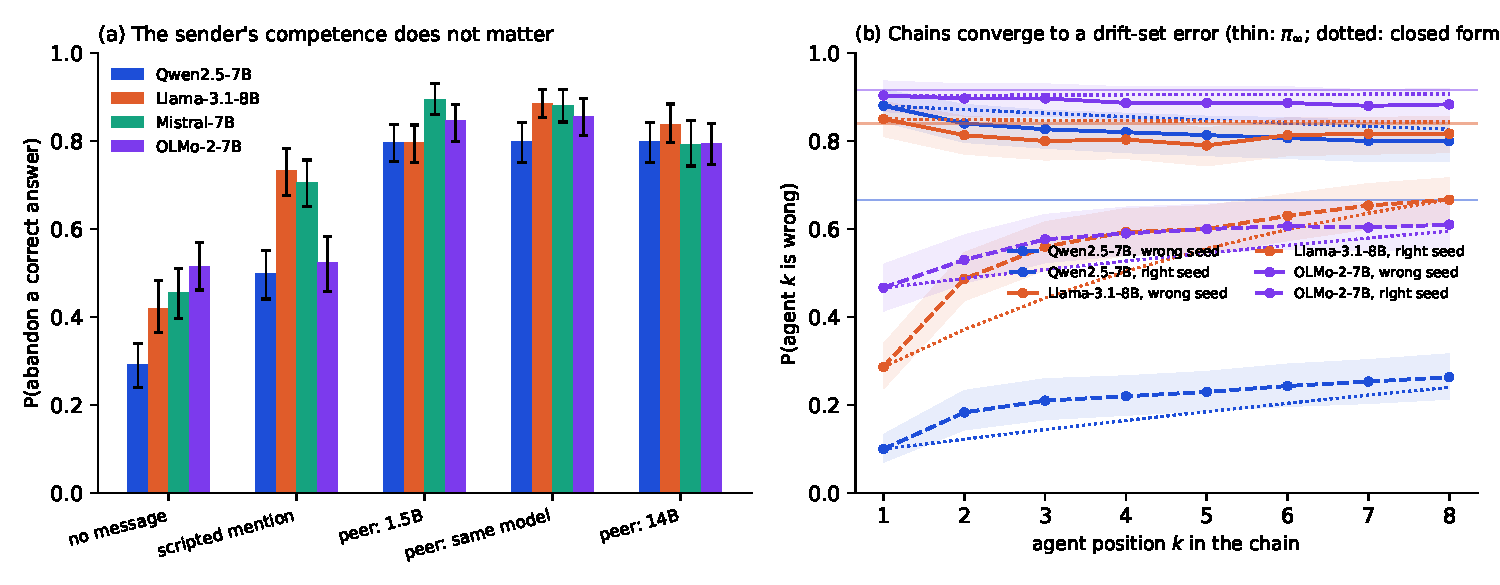
\includegraphics[width=0.86\linewidth]{../figures/fig6_contagion.pdf}
\caption{Answer contagion between agents (8-bit weights, 300 held-out questions per model). (a) An agent that holds a correct answer abandons it when a peer names an alternative, at the same rate whether the peer is a 1.5B model, the same model, or a 14B model. (b) A wrong answer forwarded through eight agents is retained at every hop; a right answer drifts toward the same long-run error. Dotted: Proposition~\ref{prop:chain} from the measured first hop; thin lines: $\piinf$. Mistral's chains \pending{re-run under the merged-turn protocol}.}
\label{fig:contagion}
\end{figure}
Everything above concerns one model and one challenger. Multi-agent systems, whether debate, self-refinement, critic pipelines or swarms of solvers, work by placing one agent's output in another's context, and the implicit promise is that agreement among agents is evidence. Assumption~\ref{ass:corpus} says otherwise: a forwarded answer is a named alternative, the strongest cue in Section~\ref{sec:control}, so a receiving agent should switch to it at the cue rate whether or not the sender knows anything, and a correct answer held by one agent should be overwritten the moment a different answer enters its context. If so, a pipeline converges to what its drift and its majority produce, regardless of which agent was right, and the only agents that keep a correct minority answer are the ones that never see the others. We test this on four open models with three pre-registered cell families (P1--P5, Appendix~\ref{app:prereg}).
\paragraph{The sender's competence does not matter.} Agent A holds an answer; a message from ``Agent B'' names a different one. When the message is written by a real peer model told to argue for the alternative, A abandons a correct answer at 0.80 / 0.80 / 0.80 (Qwen2.5-7B; a 1.5B peer / the same model / a 14B peer), 0.80 / 0.89 / 0.84 (Llama-3.1-8B), 0.89 / 0.88 / 0.79 (Mistral-7B) and 0.85 / 0.86 / 0.80 (OLMo-2-7B): spreads of 0.001, 0.09, 0.10 and 0.06 against a pre-registered threshold of 0.10 (Figure~\ref{fig:contagion}a). A reason attached to the message adds at most 0.11, and acceptance of a \emph{true} alternative stays at 0.53--0.88, so the policy is not stubbornness: it switches toward whatever is named. \pending{The same cells on the model's own generated answer.}
\paragraph{Contamination persists and clean chains drift.} Chained eight deep, each agent seeing only the previous reply, 80--90\% of agents are wrong at every hop when the seed is wrong (Table~\ref{tab:chain}): $\pww$ is 0.975--0.996. Seeded right, the chains drift toward the same fate, from 10\% to 26\% wrong (Qwen2.5-7B), 29\% to 67\% (Llama-3.1-8B) and 47\% to 61\% (OLMo-2-7B), because an agent that errs on its own is believed by every agent downstream. Proposition~\ref{prop:chain} turns the two rates into the long-run error of any pipeline built from these models, $\piinf=0.67$, $0.84$ and $0.92$, with half-lives of a seed's influence of 17, 4 and 14 hops: the pipeline forgets where an error entered while keeping the error. The pre-registered version pooled transition rates over all hops and overshot (0/8 hops inside the interval) because the seed is a bare message while later hops forward full replies; the same recursion from the measured first hop places 8/8, 6/8 and 8/8 hops inside the interval (dotted curves). We report the failure and the correction.
\begin{table}[t]\centering\scriptsize
\begin{tabular}{lcccccc}
\toprule
Model & $k=1$ & $k=4$ & $k=8$ & $\pww$ & $\pcw$ & $\piinf$ \\
\midrule
Qwen2.5-7B & .88 / .10 & .82 / .22 & .80 / .26 & .987 & .027 & .67 \\
Llama-3.1-8B & .85 / .29 & .80 / .59 & .82 / .67 & .975 & .129 & .84 \\
OLMo-2-7B & .90 / .47 & .89 / .59 & .88 / .61 & .996 & .043 & .92 \\
\bottomrule
\end{tabular}
\caption{$P(\text{agent at hop }k\text{ is wrong})$, wrong seed / right seed, with the measured rates and the stationary error of Proposition~\ref{prop:chain}.}
\label{tab:chain}
\end{table}
\paragraph{Three rules for system design.} \emph{Adding agents does not help}: with $\pi_k$ above one half, majority voting over $m$ chains makes the system wronger as $m$ grows; consensus among cue-following agents measures the cue, not the truth. \emph{Independence is the only free protection}: an agent that answers without seeing the others is right with probability $1-\pi_1$, and every exposure moves it toward $\piinf$; a correct minority answer survives only in agents that never receive the majority's. \emph{Local repair resets but does not cure}: one agent with retention $q$ resets the chain to $q$, after which the tail re-converges at rate $\lambda$, so a single robust agent protects only the hops within a half-life of it. \pending{With the STAND agent at position 2, P4 requires the downstream error to fall by $\ge0.40$; the same cells on Claude Fable 5.1 and GPT-6 Astra; 32B and 72B; bf16 replication.}

\section{Related work}
\citet{sharma2023sycophancy} traced agreeable responses to preference data; \citet{perez2022discovering}, \citet{laban2023flipflop}, \citet{stengeleskin2025pbt}, \citet{zhang2025pressuretune} and \citet{chen2024pinpoint} measured, trained against or localised the behaviour, and recent debate work finds that much apparent conformity is repetition of an alternative rather than the presence of another agent, which our identification cells confirm and extend to agents. Verbalized confidence \citep{lin2022truthfulqa,kadavath2022language} and self-evaluation predict correctness; that literature measures the monitor, and we measure whether the controller consumes it, define what consuming it would mean, and price ignoring it. The closest work finds that a model's hidden-state belief in a claim causally drives retraction \citep{aamir2026steering}; our results are complementary: the latent channel may be wired to behaviour while every explicit channel is not, and our steering null (Appendix~\ref{app:null}) is consistent with theirs. Intrinsic self-correction is unreliable \citep{huang2024selfcorrect}; our decomposition explains one mechanism, since reflection prompts inject content-free doubt. The monitoring/control distinction is from \citet{nelson1990metamemory}; we are, to our knowledge, the first to measure their coupling in language models as a quantity distinct from calibration, and the first to derive and test multi-agent contamination from a measured single-agent policy \citep{mytsyk2026bts}.

\section{Limitations}
The identification experiments inject claims as the model's prior turn; elicited-answer conditions reproduce the main patterns and the full three-cell design under elicitation is queued. All experiments are single-challenge, English and factual. The largest unquantised model is 14B \pending{32B and 72B under the identification protocol}. The trained model follows stated reliability without auditing it. The agent study measures chains only, on 8-bit weights \pending{bf16 replication}; fan-in and voting are stated as consequences of independence, not measured. Negative results are kept: steering along a declared-confidence direction is indistinguishable from random perturbation, instruction does nothing, a small synthetic DPO intervention moved nothing, the self-versus-other prediction reversed, and the pooled chain prediction failed. Exclusion rates are reported per cell with worst-case bounds.

\section{Conclusion}
Models know when they might be wrong and revise anyway. The monitor is real and improving; the controller answers to the visible surface of the conversation, and one assumption about the training objective predicts that, predicts that surfacing cannot fix it while demonstrations can at near-zero price, and predicts that the same policy makes a forwarded answer contaminate the next agent regardless of who sent it. Two uses of the pathology, survival under challenge as a calibration signal and re-asking rather than reconsidering in place, are in Appendix~\ref{app:uses}.

\subsection*{AI use statement}
We used generative AI tools for retrieval of related work, for drafting and editing code in the harness, training pipeline and Lean formalisation, and for editing prose. All design decisions, pre-registrations and claims are the authors' own and were verified against the released trial records.
\subsection*{Reproducibility statement}
All trial records, banks, harness, analysis and training code, pre-registration files with hashes, Lean proofs with build log, and \pending{trained adapters} are released. Total compute to date is roughly 160 GPU-hours on shared academic nodes plus CPU inference. No number is computed on the development slice.

\bibliography{refs}
\bibliographystyle{iclr2027_conference}

\appendix
\section{Pre-registrations}\label{app:prereg}
\pending{Verbatim: stage ladder, matched-position control, causal ladder, agent contagion (P1--P5), with hashes; the prediction that failed and the chain prediction that needed correction.}
\section{Machine-checked statements}\label{app:lean}
Propositions~\ref{prop:bayes} and \ref{prop:chain} are formalised in Lean 4 with Mathlib (\texttt{lean/RealityMonitoring/Theory.lean}, build log in \texttt{lean/BUILD\_LOG.txt}): the switching rule and its odds form, the band's non-emptiness, the fixed point, the closed form by induction, seed independence, geometric decay under positive drift, the firewall reset, and the monotone effect of a firewalled fraction; every theorem depends only on \texttt{propext}, \texttt{Classical.choice} and \texttt{Quot.sound}. \pending{Proposition~\ref{prop:regret}.}
\section{The challenge decomposition}\label{app:decomp}
The component analysis that motivated this work, recomputed in the harmful direction (the inserted claim is correct) on 450 MMLU-Pro items. Naming an alternative with no source flips 0.54--0.89 of correct claims; adding ``another source says'' adds nothing in the Llama family and OLMo-2 and 0.21--0.30 in Qwen and Mistral; content-free doubt alone flips 0.14--0.82. A note that Qwen2.5-7B's answer is ninety percent reliable raises abandonment as much as a thirty-percent warning \pending{harmful-direction recompute}.
\begin{figure}[h]\centering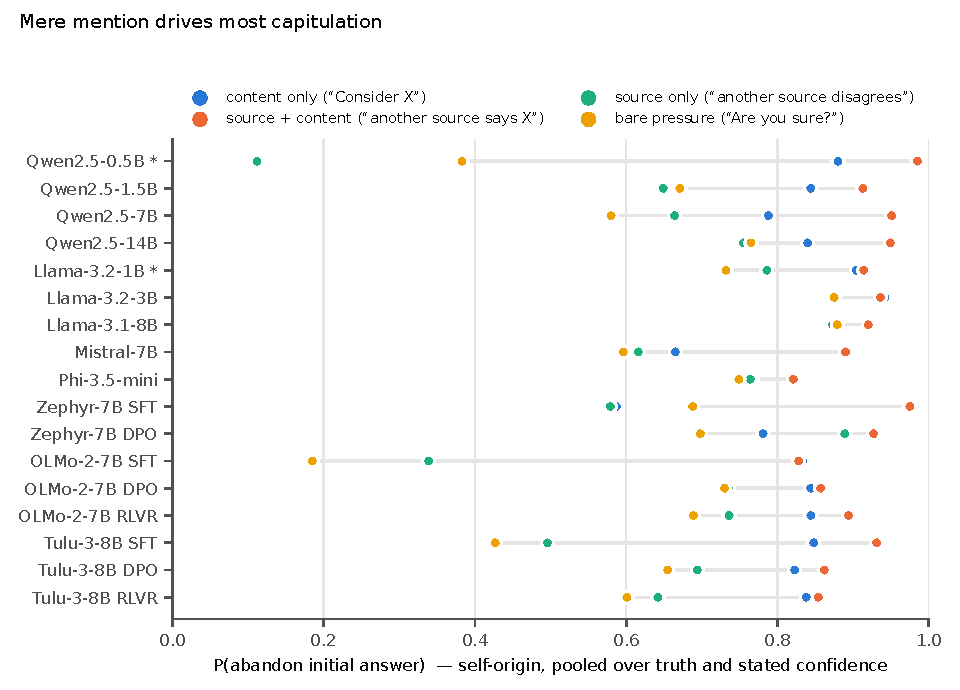
\includegraphics[width=0.66\linewidth]{../figures/fig1_decomposition.pdf}\caption{Harmful abandonment by challenge kind across checkpoints.}\label{fig:decomp}\end{figure}
\begin{table}[h]\centering\footnotesize\setlength{\tabcolsep}{4pt}
\begin{tabular}{lcccccc}
\toprule
Checkpoint & sourced counter & bare counter & source only & pressure & source effect & excluded \\
\midrule
Llama-3.2-3B & .88 & .89 & .80 & .82 & $-$.01 & .10 \\
Llama-3.1-8B & .85 & .86 & .78 & .80 & $-$.01 & .06 \\
Qwen2.5-7B & .90 & .62 & .50 & .40 & .28 & .02 \\
Qwen2.5-14B & .90 & .69 & .57 & .57 & .21 & .01 \\
Mistral-7B & .85 & .55 & .54 & .48 & .30 & .11 \\
Phi-3.5-mini & .64 & .59 & .57 & .55 & .05 & .15 \\
OLMo-2-7B-SFT & .79 & .80 & .26 & .14 & $-$.01 & .04 \\
OLMo-2-7B-DPO & .75 & .74 & .62 & .59 & .01 & .10 \\
OLMo-2-7B-Instruct (RLVR) & .83 & .76 & .65 & .57 & .07 & .04 \\
T\"ulu-3-8B-SFT & .88 & .77 & .41 & .34 & .11 & .02 \\
T\"ulu-3-8B-DPO & .76 & .70 & .55 & .50 & .06 & .06 \\
T\"ulu-3-8B (RLVR) & .75 & .73 & .50 & .46 & .02 & .03 \\
Zephyr-7B-SFT & .96 & .54 & .51 & .62 & .42 & .05 \\
Zephyr-7B-DPO & .88 & .69 & .85 & .65 & .19 & .04 \\
\bottomrule
\end{tabular}
\caption{Harmful abandonment by challenge kind, self origin, parseable trials; source effect $=$ sourced $-$ bare.}
\end{table}
\section{Training-stage ladders}\label{app:stage}
\begin{figure}[h]\centering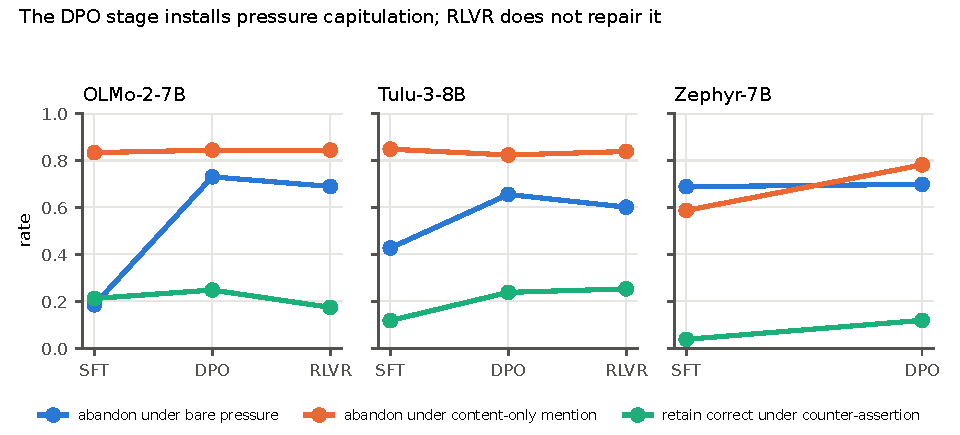
\includegraphics[width=0.8\linewidth]{../figures/fig3_stage_ladder.pdf}\caption{Pressure capitulation along the OLMo-2, T\"ulu-3 and Zephyr lineages.}\end{figure}
\section{The bidirectional firmness intervention}\label{app:firm}
\pending{Training data, held-out phrasings, per-seed cells, boundaries.}
\section{Surfacing null, full table}\label{app:surf}
\pending{Per-value curves for six models, latent and surfaced.}
\section{Null and negative results}\label{app:null}
\pending{Steering, instruction, synthetic DPO dose-response.}
\section{The causal ladder and STAND}\label{app:stand}
\begin{figure}[h]\centering
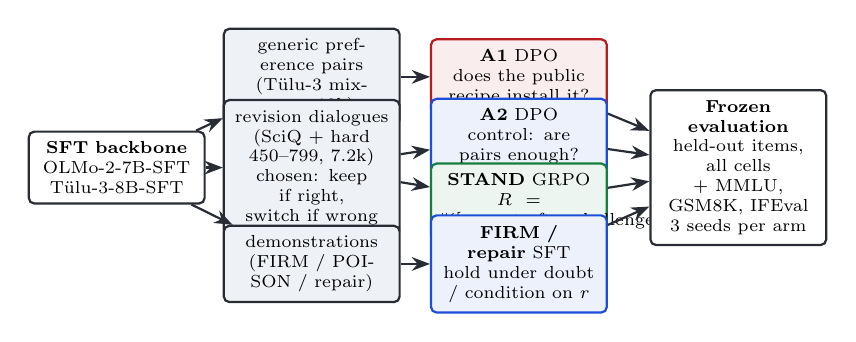
\begin{tikzpicture}[x=0.86cm,y=0.8cm,>=Stealth,font=\scriptsize,scale=0.9,every node/.style={transform shape}]
\tikzset{st/.style={draw=ink,rounded corners=2pt,fill=white,inner sep=4pt,align=center,text width=2.2cm,thick},
  data/.style={st,fill=soft},arm/.style={st,fill=rel!8,draw=rel},fix/.style={st,fill=evid!8,draw=evid},bad/.style={st,fill=cue!8,draw=cue},arr/.style={->,thick,draw=ink}}
\node[st] (sft) at (0,0) {\textbf{SFT backbone}\\OLMo-2-7B-SFT\\T\"ulu-3-8B-SFT};
\node[data] (gen) at (3.2,1.6) {generic preference pairs\\(T\"ulu-3 mixture, 10k)};
\node[data] (rev) at (3.2,0) {revision dialogues\\(SciQ + hard 450--799, 7.2k)\\chosen: keep if right,\\switch if wrong};
\node[data] (dem) at (3.2,-1.7) {demonstrations\\(FIRM / POISON / repair)};
\node[bad] (a1) at (6.6,1.6) {\textbf{A1} DPO\\does the public recipe install it?};
\node[arm] (a2) at (6.6,0.55) {\textbf{A2} DPO\\control: are pairs enough?};
\node[fix] (a3) at (6.6,-0.6) {\textbf{STAND} GRPO\\$R=\mathbb{1}[\text{correct after challenge}]$};
\node[arm] (d2) at (6.6,-1.7) {\textbf{FIRM / repair} SFT\\hold under doubt / condition on $r$};
\node[st] (ev) at (10.2,0) {\textbf{Frozen evaluation}\\held-out items, all cells\\+ MMLU, GSM8K, IFEval\\3 seeds per arm};
\draw[arr] (sft)--(gen);\draw[arr] (sft)--(rev);\draw[arr] (sft)--(dem);
\draw[arr] (gen)--(a1);\draw[arr] (rev)--(a2);\draw[arr] (rev)--(a3);\draw[arr] (dem)--(d2);
\draw[arr] (a1)--(ev);\draw[arr] (a2)--(ev);\draw[arr] (a3)--(ev);\draw[arr] (d2)--(ev);
\end{tikzpicture}
\caption{The causal ladder. Every arm starts from a pre-preference checkpoint, trains with LoRA (rank 64), is merged, and is scored by the same frozen harness and capability suites.}
\end{figure}
\begin{algorithm}[h]
\caption{STAND, one GRPO step}\label{alg:stand}
\begin{algorithmic}[1]
\Require policy $\pi_\theta$ (SFT backbone $+$ LoRA), reference $\pi_{\mathrm{ref}}$, challenge dialogues $\{(q_i,c_i,x_i,a^{*}_i)\}$ outside the evaluation set, group size $G=8$, KL weight $\beta$
\For{each dialogue $i$}
  \State sample $y_{i,1..G}\sim\pi_\theta(\cdot\mid q_i,c_i,x_i)$ (128 tokens, temperature 1)
  \State $R_{i,g}\gets\mathbb{1}[\mathrm{final}(y_{i,g})=a^{*}_i]+0.1\cdot\mathbb{1}[\text{ends with a \texttt{FINAL:} line}]$
  \State $\hat A_{i,g}\gets(R_{i,g}-\mathrm{mean}_g R_{i,\cdot})/\mathrm{std}_g R_{i,\cdot}$
\EndFor
\State $\theta\gets\theta+\eta\nabla_\theta\frac{1}{|B|}\sum_{i,g}\big[\tfrac{\pi_\theta(y_{i,g})}{\pi_{\theta_{\mathrm{old}}}(y_{i,g})}\hat A_{i,g}-\beta\,\mathrm{KL}(\pi_\theta\|\pi_{\mathrm{ref}})\big]$; every fifth batch, one epoch of plain question answering (replay)
\end{algorithmic}
\end{algorithm}
\section{Two uses for the pathology}\label{app:uses}
Because revision responds to the one epistemic variable models weight, the truth of their own claim, an answer's survival under a standardized battery of challenges carries information about its correctness: survival rate as a confidence score beats stated confidence in sixteen of nineteen checkpoints (Qwen2.5-7B 0.71 vs 0.66; Qwen2.5-14B 0.77 vs 0.70; Qwen2.5-32B 0.76 vs 0.73; Phi-3.5 0.75 vs 0.58), with no training, logit access or calibration set. And on questions a model initially answers correctly, an in-context request to reconsider after a false counter leaves accuracy at 0.00--0.08, while re-asking in a fresh context restores the answer; under greedy decoding the identical re-ask is a determinism check, so the informative quantity is the near-zero in-context number \pending{against paraphrased re-asks under sampling}.
\section{Per-checkpoint tables and figures}\label{app:tables}
\begin{figure}[h]\centering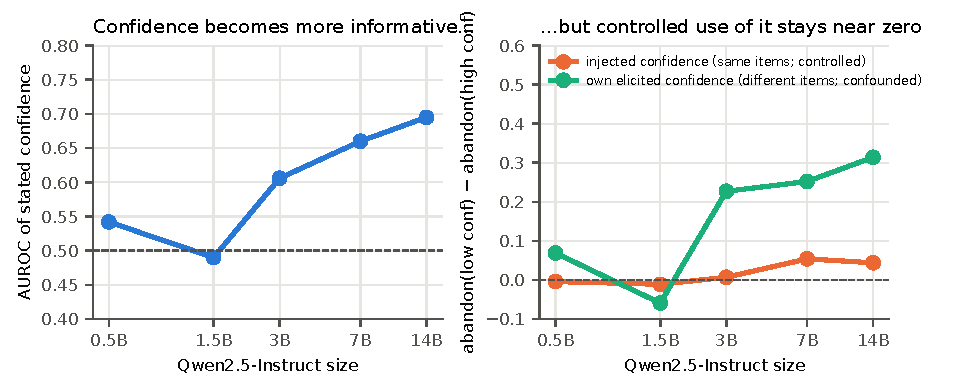
\includegraphics[width=0.85\linewidth]{../figures/fig2_scissors.pdf}\caption{Elicited confidence becomes informative with scale while matched behavioural use of reliability wording stays near zero.}\end{figure}
\begin{figure}[h]\centering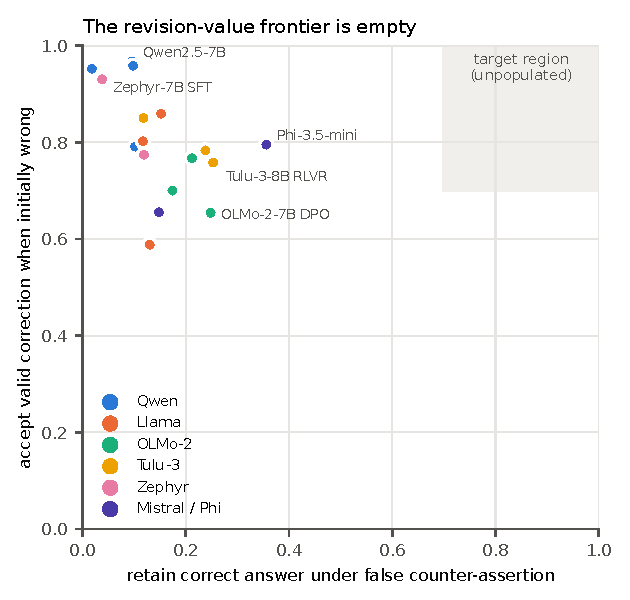
\includegraphics[width=0.55\linewidth]{../figures/fig4_frontier.pdf}\caption{The retain/accept frontier is empty for every measured checkpoint \pending{trained arms as arrows}.}\end{figure}
\pending{Beneficial-direction tables, exclusion fractions and worst-case bounds, matched-position estimates per checkpoint, capability deltas per trained arm, all agent cells.}
\end{document}
